\documentclass[../thesis.tex]{subfiles}

\begin{document}

\chapter{Implementierung}
\label{chp: implementierung}

Die Implementierung lässt sich in drei verschiedene Bestandteile aufteilen, welche in den folgenden Abschnitten näher erläutert werden.

\section{Datenbank}

Die Klasse \texttt{database} dient zur Bereitstellung und Speicherung aller benötigten Daten. Diese Daten beinhalten sowohl die der Experimente, als auch die des Modells. Die Klasse Datenbank erzeugt im gleichnamigen Ordner für jedes Gemisch eine eigene Datei, in der alle Daten im \textit{.json} Format abgelegt sind. Der beispielhafte Aufbau einer Gemischdatei ist in \autoref{code: beispielgemisch} dargestellt.

\definecolor{codehighlight}{rgb}{0.95,0.8,0.8}
\lstinputlisting[language=Python, caption=Gemischdatei Beispiel, basicstyle=\fontsize{7}{8}\selectfont\ttfamily
]{./code/gemischbeispiel.json}
\label{code: beispielgemisch}

Der Schlüssel \texttt{BAC} dient der Klassifizierung des Gemisches, wie in \autoref{sec: gemischklassifikation} beschrieben. Das Tabellenblatt auf dem die Daten in der Originaldatei zu finden sind als Wert des Schlüssels \texttt{sheet} gespeichert. Analog zum Aufbau der Originaldatei werden unter den weiteren Schlüsseln die Daten der gemessenen Größen gespeichert. Alle Messreihen werden als Liste unter dem Variablennamen gespeichert.

Eine Messreihe ist durch ihre Quelle unter dem Punkt \texttt{reference}, die Parameter der Messung unter dem Punkt \texttt{params}, und die Messdaten unter dem Punkt \texttt{measurements} charakterisiert.

Somit stehen alle experimentellen Daten in computerlesbaren Format bereit.

\section{Modell}

Die Klasse \texttt{model} dient dazu die Daten des Modells bereitzustellen, damit diese anschließend mit den experimentellen Daten verglichen und bewertet werden können.

Der Ablauf der Berechnung für ein Gemisch ist in \autoref{fig: model_berechnung} gezeigt.

\begin{figure}[htb]
	\centering
	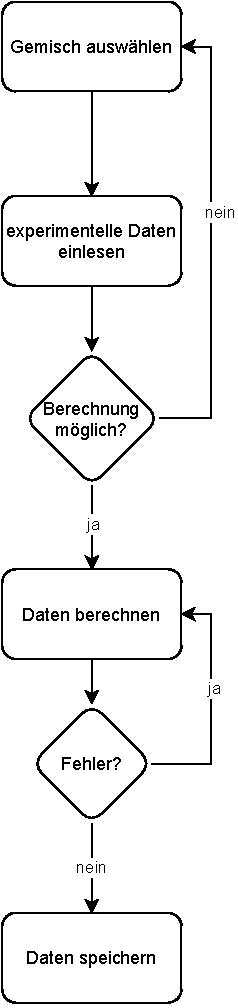
\includegraphics[scale=0.6]{berechnung_model}
	\caption{Ablauf Berechnung Model}
	\label{fig: model_berechnung}
\end{figure}

Für jedes Gemisch werden die folgenden Schritte für jede zu berechnende Größe durchgeführt. Als erster Schritt wird das zu berechnende Gemisch festgelegt. Anschließend werden alle vorhandenen experimentellen Daten aus der entsprechenden \texttt{.json} Datei eingelesen. Die hier eingelesen Daten bestimmen was das Modell berechnen soll. Es werden alle Größen, die für das Gemisch gefunden wurden nacheinander berechnet. Bevor das Modell aufgerufen wird wird getestet, ob das Modell die Daten für das Gemisch überhaupt berechnen kann. Dieser Test basiert meistens auf den Parametern die für das Modell vorhanden sind. Ist ein Stoff an dem Gemisch beteiligt für das das Modell keine Parameter hat kann das Modell keine Ergebnisse berechnen. Dieses Gemisch wird übersprungen.
Kann das Modell die geforderten Daten berechnen wird es aufgerufen und wenn kein Fehler bei der Berechnung auftritt werden die Daten gespeichert. Andernfalls wird der versucht den nächsten Datenpunkt zu berechnen. Die Datei mit den Berechnungsergebnissen des Modells hat den gleichen Aufbau, wie die der experimentellen Daten aus \autoref{code: beispielgemisch}

\section{Bewertung}

\end{document}
